\subsubsection{Estudo puramente geométrico}
A abordagem puramente geométrica é uma análise do espaço de trabalho do
manipulador na pá. Utiliza os manipuladores da pesquisa de mercado como
objetos deste estudo e leva em consideração as dimensões da
pistola, o ângulo máximo e mínimo para o revestimento ($90^o \pm 60^o$), e a
distância mínima de 230 mm entre a pistola e a pá. É um estudo simplificado por não considerar as possíveis colisões com o ambiente, assumir
que a pá está contida em um plano (projeção, objeto 2D) e considerar o espaço
de trabalho do manipulador simétrico. A abordagem geométrica foi desenvolvida
com o auxílio do software Geogebra.

Primeiramente, o espaço de trabalho do manipulador é simplificado
como a maior esfera que pode ser contida dentro de seu espaço de
trabalho real. O raio dessa esfera é calculado e considerado como o
alcance do manipulador. A pá é, então, projetada em planos, como mostra a
figura~\ref{fig::paplanos}, e o plano direito corta a esfera do espaço de
trabalho do manipulador. 

Essa abordagem é abordado de maneira específica a seguir, considerando cada
manipulador da pesquisa de mercado.

\begin{figure}[h!]	
	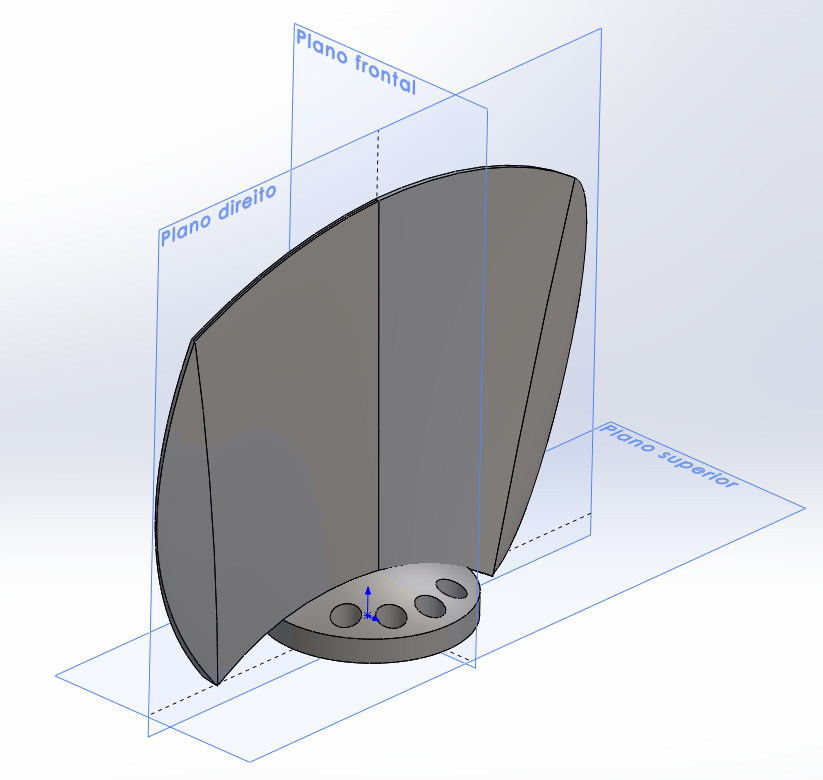
\includegraphics[width=\columnwidth]{figs/bighatch/PaPlanos.PNG}
	\caption{Ilustração das projeções da pá em planos.}
	\label{fig::paplanos}
\end{figure}

\paragraph{KR 10 R1100 sixx WP (Kuka)}
A figura~\ref{fig::kukageom} ilustra a interseção do espaço de trabalho
simplificado do manipulador Kuka KR10 e a projeção da pá. No
caso do Kuka KR 10 R1100, o raio da esfera é aproximado a $\overline{OB^i} = $
alcance do manipulador + comprimento da pistola + 230 mm $= $. 

\begin{figure}[h!]	
	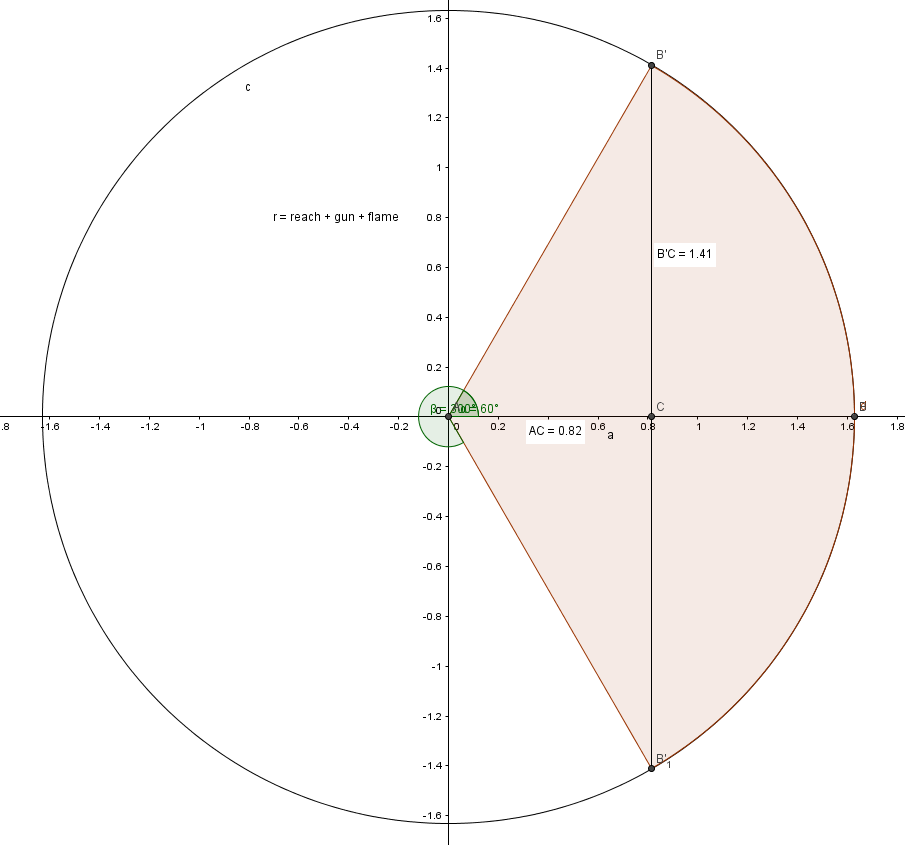
\includegraphics[width=\columnwidth]{figs/bighatch/kukageom.jpg}
	\caption{Ilustração da interseção do espaço de trabalho simplificado do
	manipulador Kuka KR10 e a projeção da pá.}
	\label{fig::kukageom}
\end{figure}

\paragraph{MH12 (Motoman)}

\begin{figure}[h!]	
	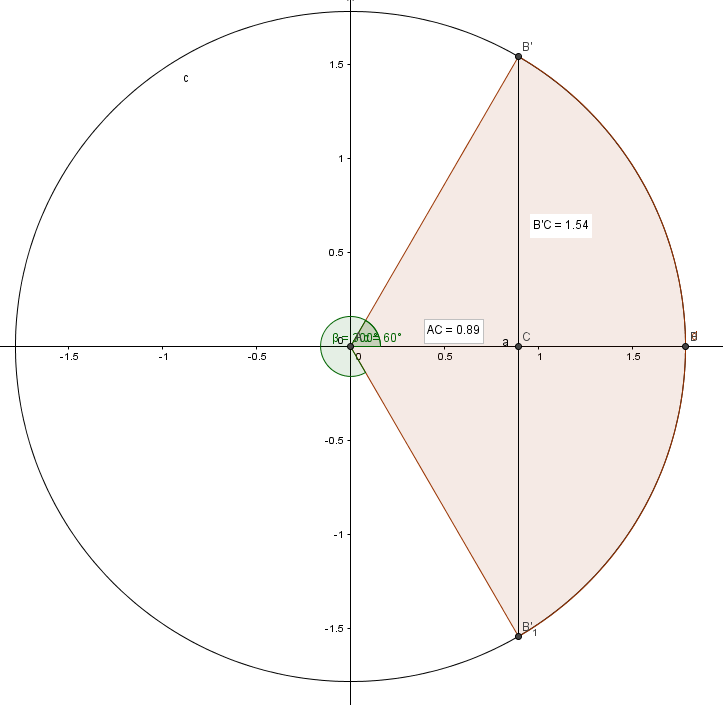
\includegraphics[width=\columnwidth]{figs/bighatch/motomangeom.jpg}
	\caption{Ilustração da interseção do espaço de trabalho simplificado do
	manipulador Motoman MH12 e a projeção da pá.}
	\label{fig::motomangeom}
\end{figure}